\section{Validating the Generated DYMO Code}
\label{sec:dymoexperiments}
In this section we give an impression of the generated code from the DYMO model, and explain the manual work that needs to be done in order to be able to execute the code. We also validate the generated Erlang code by using a simple network simulator to simulate the transmission of messages in a MANET. The implementation is executed, and the routing tables are inspected to verify that the connections were correctly established.

\subsection{Generating the Code and Implementing the Functions}

Generating the code from the DYMO model yields the modules shown in Table~\ref{table:gencodestat}. All these modules can be found in appendix \ref{appsec:dymocode_unmod}. We have listed lines of code (L.O.C.) for each module -- in total we generated 563 lines of code. Since we do not support automatic translation from CPN ML to Erlang, we had to manually implement various Erlang expressions and functions on the basis of the corresponding CPN ML code. These CPN ML expressions are carried along as comments in the generated code. The comments are placed where the expression should be used, thus the structure of the program is preserved. Implementing the functions (12 in total) in Erlang is an easy task, because of the similarity between Erlang and CPN ML. In appendix \ref{appsec:dymocode_mod} we show the modified modules. We spent approximately 12 person-hours modifying the generated code, but the time spent would be eliminated if we had an automatic translation from CPN ML to Erlang. 

\begin{table}
\vspace*{1em}
\begin{center}
\begin{tabular}{llllll}
    Module name  	& & L.O.C.	& & Functions to implement \\  \noalign{\smallskip}\hline\noalign{\smallskip}
	system.erl 		& & 20	& & 0 \\	
	buffer.erl 		& & 36  & & 0 \\
	shared.erl 		& & 16 	& & 0 \\
	initiator.erl 	& & 116	& & 1 [createRREQ] \\
	receiver.erl  	& & 116 & & 7 [isOwnMessage, isNewRoute, \dots] \\
	                                % isStale, isLoopPossible,isInferior, isSuperiorm, updateRouteEntry] \\
	processer.erl 	& & 111 & & 4 [isRREP, isRREQ, isTarget, \dots] \\
									%isRREP, isRREQ, isTarget, createRREP
	establishchecker.erl & & 126  & & 0 \\
	network.erl 	& & 22	& & 0 \\	
	   
	\noalign{\smallskip}\hline\noalign{\smallskip}
	Total & & 563 & & 12
	\\ \noalign{\smallskip}\hline\noalign{\smallskip}
\end{tabular}
\vspace*{1em}
\end{center}   
\caption{The Generated Modules from the DYMO Protocol}
\label{table:gencodestat}
\end{table} 

\begin{figure}[b!]
\begin{verbatim}
  rreq_target(Env) -> 
  Msg = Env#environment.message_for_processing,
  Ip = Env#environment.own_process_ip_address,
  routing_table ! {get, self()},
  receive 
    Rota -> 
      Rota
  end,
  seqnum ! {get, self()},
  receive 
    Seqnum -> 
      Seqnum
  end,
  NewEnv = Env#environment {},
  routing_table ! {set, Rota},
  seqnum ! {set, Seqnum},
  Id1 = 1,
  Receiver1 = list_to_atom("network_ID" ++
  integer_to_list(Id1) ++ "_dymo_to_network"),
  Receiver1 ! {send, %% createRREP(ip, msg, rota, seqNum)
  undefined},
  receive_incoming_message(NewEnv).
\end{verbatim}
\end{figure}

To give an impression of the task of manually implementing the CPN ML functions we take a look at some of the generated code. In Listing~\ref{fig:rreqtargetcode} we show the unmodified generated code for the \code{rreq\_target} function in the \code{processer} module. The \code{rreq\_target} function is called when a node discovers that it is the target of a route request message. A RREP message needs to be created in order to make a reply. In the CPN model the reply message is created by a CPN ML function. In line 20 of Listing~\ref{fig:rreqtargetcode} we see the CPN ML function \code{createRREP} as a commment. What needs to be done is to translate the CPN ML function \code{createRREP} to an equivalent Erlang function.

We have done this by replacing line 20 and 21 with the single line shown in Listing~\ref{fig:createRREPcall}.

\begin{figure}[h!]
\begin{verbatim}
Receiver1 ! {send, createRREP(Ip, Msg, Rota, SeqNum)},
\end{verbatim}
\end{figure}

The difference is that the comment character (\%) has been removed and the casing of the arguments to the function has been changed. Notice, that the function \code{createRREP} is given some arguments. These arguments has either been extracted from the environment or read from global variables. What is left to be done is implementing the function \code{createRREP}.

\begin{figure}[h!]
\begin{verbatim}
createRREP(Msg, Own_ip, Rota, SeqNum) ->
  Entry = util:get_entry(Msg#message.orig_addr, Rota),
  Next_hop_address =
             Entry#routing_table_entry.next_hop_address,
  #message {src = Own_ip, dest = Next_hop_address,
            target_addr = Msg#message.orig_addr, 
            orig_addr = Own_ip, orig_seqnum = SeqNum, 
            hop_limit = 5, dist = 1, msg_type = 'RREP'}.
\end{verbatim}
\end{figure}

The created Erlang function \code{createRREP} (shown in Listing~\ref{fig:createRREPfunction}) first extracts the entry of the originator of the request from the routing table. Then the next hop address is found in the entry. This information, along with information from the message and the sequence number, is used to create the reply message according to the DYMO specification.

\subsection{Setting-up a Network Simulation}
In order to execute more than one node running the generated DYMO implementation, we use the \emph{distributed Erlang system} which is a mechanism in Erlang allowing a number of Erlang systems to communicate over a network. It consists of a number of independent Erlang runtime systems. Each runtime system is called an \code{Erlang node}, and each node executes the same generated DYMO code. An advantage of using the distributed Erlang system is that each node has its own \emph{name space}, thus all the generated names of process instances does not have to be modified. For instance, in the \code{system} module all the registered names can remain unchanged.

The processes running the DYMO implementation on different Erlang nodes do not communicate directly with each other. Instead they communicate through a \emph{network simulator} process running on a separate Erlang node. The stub code for the network simulator was generated directly from the \code{network} process partition of the DYMO ProPCPN model (see bottom of Fig.~\ref{fig:systemmodule}). This means that the generated \code{initiator} and \code{processer} processes sends messages to the network by sending them to the buffer of the \code{network} process. Also, the \code{receiver} process is ready to receive messages from the network through its buffer. The network simulator process implements a simple MANET with a static topology where both unicast and multicast is supported. The topology is implemented by using an adjacency list representation. For each node there is a list specifying which nodes are in direct transmission range. When the destination address in a message is a unicast address it is passed directly to the node with the given address, and when a message contains a multicast address the message is passed to each node in the adjacency list of the sending node.

\subsection{Results of the Execution}
The generated DYMO code was then executed in the distributed environment. To monitor the behaviour of the program, each node prints its own routing table, which can then be inspected to verify that the expected routes were established. The first tests were done with topologies containing two and three nodes, and we found that routes were established as expected.

The generated DYMO code was then executed in the topology shown in Fig.~\ref{fig:mscrreq} with five nodes where node 1 is requesting a route to node 5. After the execution we inspected the routing tables of the nodes in the network. Node 1 had the following routing table:

\begin{center}
\begin{tabular}{|c|c|c|c|}
\hline
\multicolumn{4}{|c|}{\textbf{Routing table of node 1}} \\
\hline
\textit{Address} & \textit{SeqNum} & \textit{NextHopAddress} & \textit{Dist} \\
\hline
node 5 & 1 & node 2 & 2 \\
\hline
\end{tabular}
\end{center}

\noindent As we can see, node 1 has an entry for a route to node 5 through node 2 with a distance of 2. The routing table for node 2 was as follows:

\begin{center}
\begin{tabular}{|c|c|c|c|}
\hline
\multicolumn{4}{|c|}{\textbf{Routing table of node 2}} \\
\hline
\textit{Address} & \textit{SeqNum} & \textit{NextHopAddress} & \textit{Dist} \\
\hline
node 1 & 1 & node 1 & 1 \\
\hline
node 5 & 1 & node 5 & 1 \\
\hline
\end{tabular}
\end{center}

\noindent Node 2 has two entries for routes in its routing table, namely for node 1 and node 5. These entries show, that node 2 can send messages directly to both node 1 and node 5. This means that other nodes can send messages to node 1 and node 5 through node 2. Finally, the routing table on node 5:

\begin{center}
\begin{tabular}{|c|c|c|c|}
\hline
\multicolumn{4}{|c|}{\textbf{Routing table of node 5}} \\
\hline
\textit{Address} & \textit{SeqNum} & \textit{NextHopAddress} & \textit{Dist} \\
\hline
node 1 & 1 & node 2 & 2 \\
\hline
\end{tabular}
\end{center}

\noindent This routing table has a single entry for a route to node 1 through node 2 with a distance of 2. It can be seen that the route between node 1 and node 5 was correctly established in both directions. 

\begin{figure}
\centering
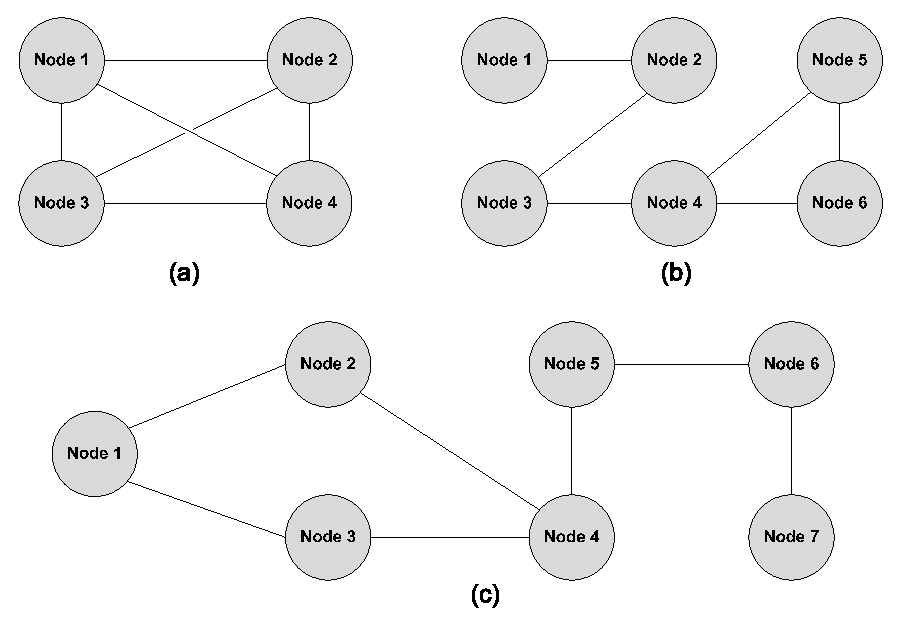
\includegraphics[scale=0.8]{dymo/graphics/topologies.eps}
\caption{Topologies to test the generated DYMO code}
\label{fig:topologies}
\end{figure}

To make sure that every part of the generated code at some point has been executed we have executed the generated DYMO code in the topologies shown in Fig.~\ref{fig:topologies}. In topology (a), node 1 makes a route request for node 4. This has the effect that all functions used to determine the usefulness of routing information is executed at least once. In topology (b), node 1 is requesting a route to node 6. This shows that the nodes are capable of establishing a route which consists of four hops. To further investigate the length of the routes we constructed topology (c), where node 1 is requesting a route to node 7. This test the part of the code that deals with the hop limit of a message. The shortest route between node 1 and node 7 has four intermediate nodes. When executing the protocol, where the messages contain a hop limit of four, the route could not be established. By increasing the hop limit to five the route was established through the four intermediate hops. Having all parts of the generated code executed with the expected outcome builds confidence in the correctness of the generated code.
